%%%%%%%%%%%%%%%%%%%%%%%%%%%%%%%%%%%%%%%%%%%%%%%%%%%%%%%%%%%%%%%%%%%%%%%%%%%%%%%%%%%%%%%%%%%%%%%%%%%%%%%%%%%%%%%%%%%%%%%%%%%%%%%%%%%%%%%%%%%%%%%%%%%%%%%%%%%%%%%%%%%%%%%%%%%%%%%%%%%%%%%%%%%%%%%%%%%%%%%%%%%%%%%%%%%%%%%%%%%%%%%%%%%%%%%%%
\iffalse\fi
%%%%%%%%%%%%%%%%%%%%%%%%%%%%%%%%%%%%%%%%%%%%%%%%%%%%%%%%%%%%%%%%%%%%%%%%%%%%%%%%%%%%%%%%%%%%%%%%%%%%%%%%%%%%%%%%%%%%%%%%%%%%%%%%%%%%%%%%%%%%%%%%%%%%%%%%%%%%%%%%%%%%%%%%%%%%%%%%%%%%%%%%%%%%%%%%%%%%%%%%%%%%%%%%%%%%%%%%%%%%%%%%%%%%%%%%%

\documentclass[12pt, letterpaper]{article}

\usepackage{../../../../texmf/mathematics}

\title{\color{BlueGreen}\textbf{Arithmetical Logical Unit Design}}
\author{
\textcolor{OliveGreen}{Laz\u{a}r-Iulian Boariu} \\
\textcolor{Lavender}{Maria-Alexia Crișan}
                                        }
\date{18th of April, 2025} 

\begin{document}

\maketitle

\newpage

\tableofcontents

\newpage

\Section{1}{Abstract}

This project presents the design and implementation of an \textcolor{cyan}{Arithmetic Logic Unit} (ALU)
capable of performing both logical and arithmetic operations on two 8-bit operands. The ALU supports basic logical operations including
\textcolor{red}{AND}, \textcolor{red}{OR}, and \textcolor{red}{XOR},
as well as fundamental arithmetic operations such as
\textcolor{BurntOrange}{addition}, \textcolor{BurntOrange}{subtraction}, \textcolor{purple}{multiplication}, and \textcolor{purple}{division}.
The goal of this project is to show how these basic operations can be combined into a simple digital system.
The project was developed as part of the \textcolor{cyan}{Calculatoare Numerice} course.

\Section{2}{Finite State Diagram}

\begin{center}
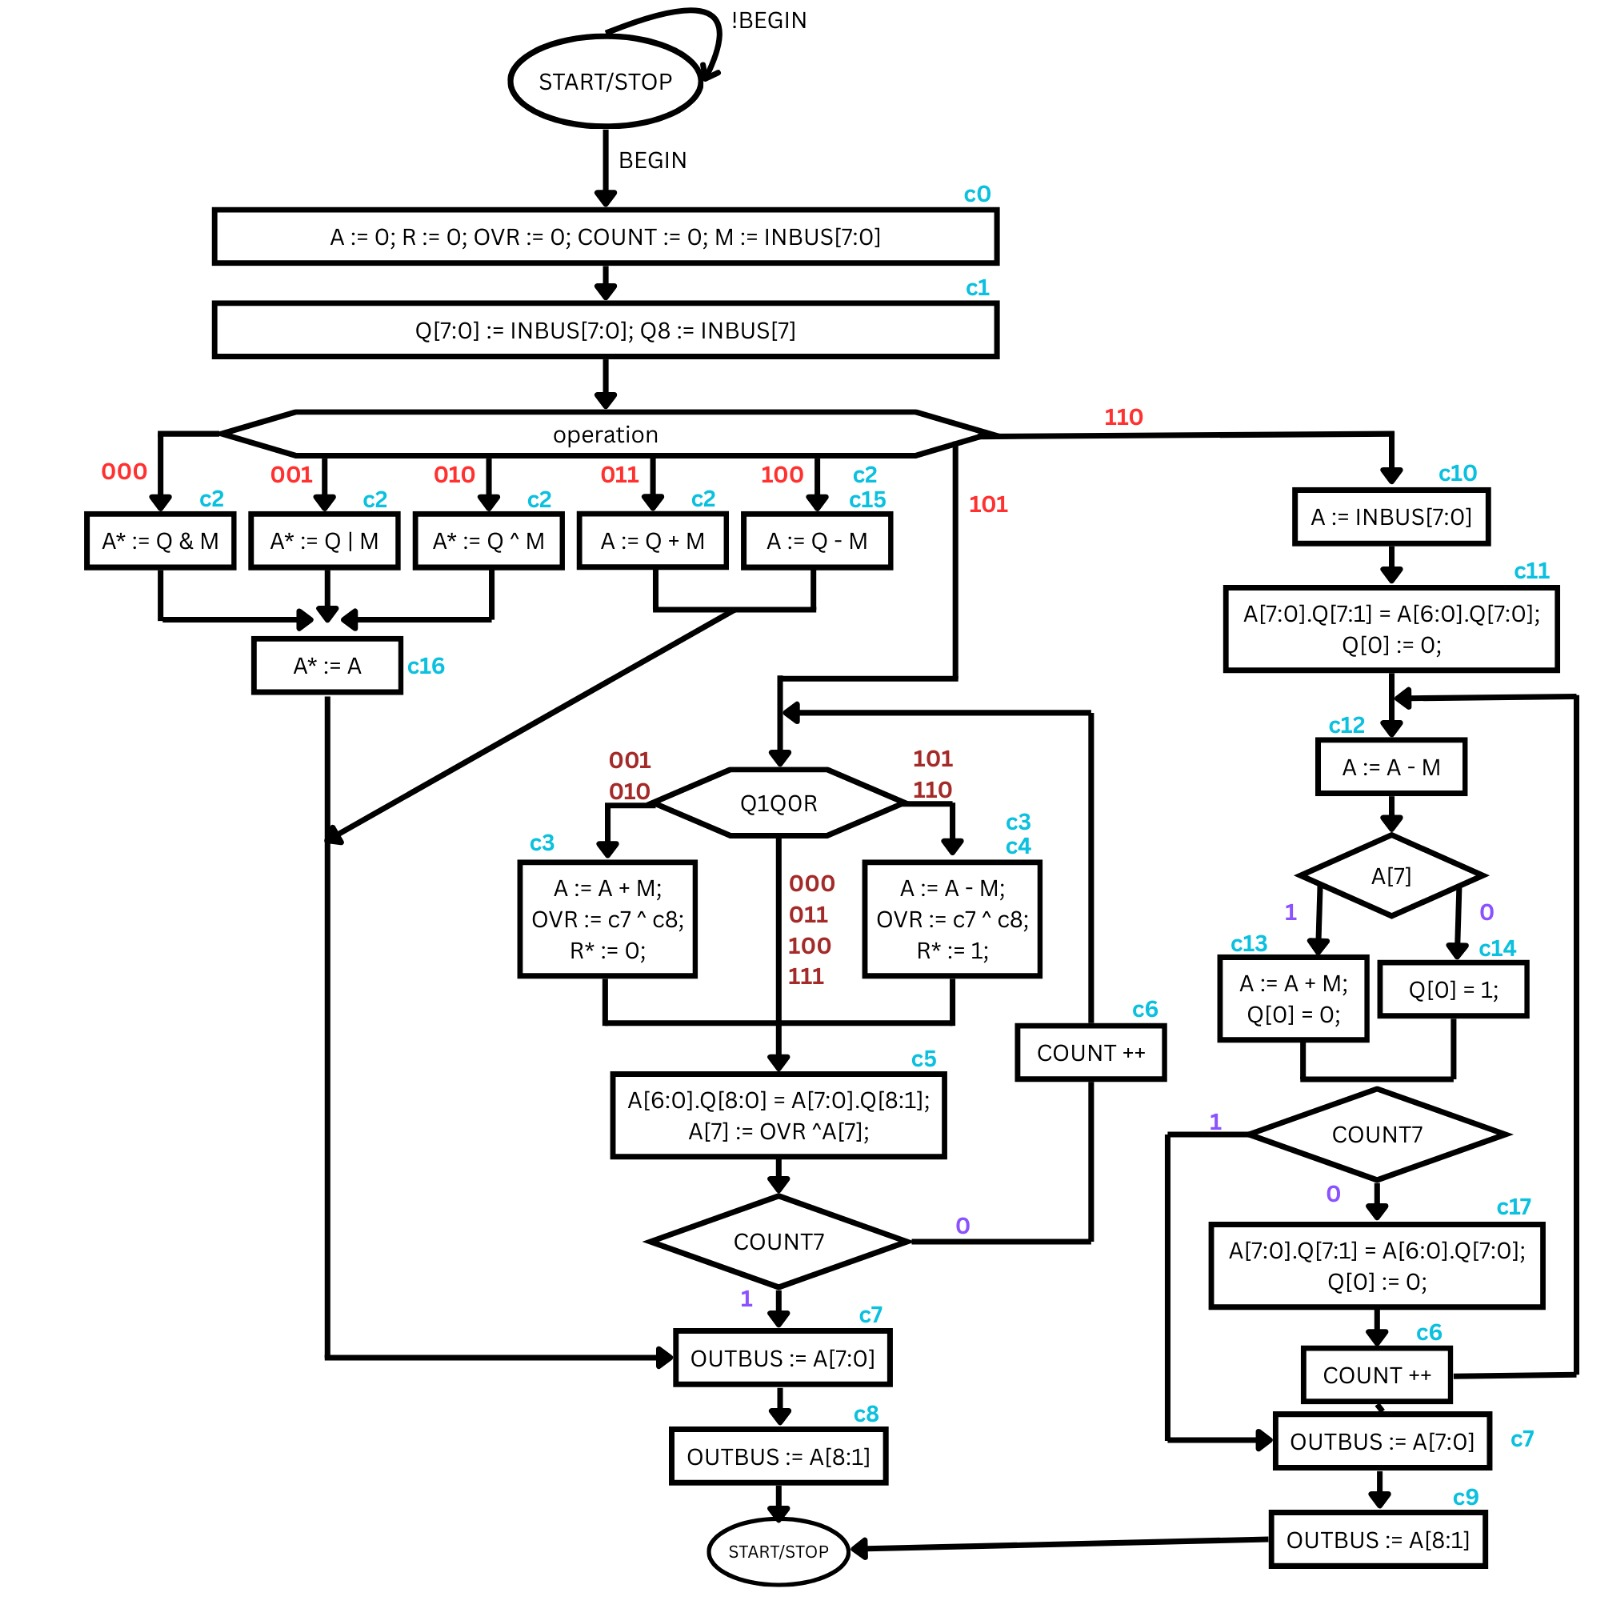
\includegraphics[scale=0.3]{Documentation/FSM}
\end{center}

The diagram illustrates the overall behavior of the ALU, detailing the steps involved in processing data and selecting the appropriate operation based on the provided operation code.\\


The design begins with the initialization of registers and variables, including the two 8-bit operands (Q and M), a remainder register (R), overflow flag (OVR), and a counter.
The control logic then decodes the operation code to determine which operation to execute—logical (AND, OR, XOR) or arithmetic (addition, subtraction, multiplication, division).
Each operation follows a specific path in the flowchart, with conditional branches guiding the transitions between processing stages.\\


Multiplication is implemented using the Modified Booth algorithm, which improves performance by reducing the number of partial products, and is triggered by specific control signals. Similarly, division is handled using the
Restoring Division method, as shown on the right side of the diagram. This method involves conditional subtraction and shifting, iteratively refining the quotient and remainder.\\


The process continues until the counter reaches its limit, after which the final result is written to the output bus. The flowchart provides a structured overview of how the ALU manages complex operations in a controlled and
sequential manner.\\

\Section{3}{Algorithms Used}

\textcolor{RoyalBlue}{\textbf{Modified Booth Multiplication}}

The Modified Booth algorithm is an efficient technique used for signed binary multiplication. It works by encoding the multiplier in groups of three bits, allowing the algorithm to reduce the number of partial products that need to
be generated and added. Instead of performing a simple shift-and-add for every bit of the multiplier, Booth encoding identifies patterns and replaces them with fewer arithmetic operations, such as subtracting or addition. This
method increases speed and reduces the hardware complexity of the multiplier, making it especially useful for larger word sizes or performance-critical designs.\\

\textcolor{CarnationPink}{\textbf{Restoring Division}}

Restoring division is a classic algorithm used for performing binary division by sequentially subtracting the divisor from the partial remainder. At each step, the dividend is shifted left, and the divisor is subtracted from the
current remainder. If the result is positive, the subtraction was valid, and the quotient bit is set to 1. If the result is negative, the original remainder is restored by adding the divisor back, and the quotient bit is set to 0.\\

\Section{4}{ALU Design}

\begin{center}
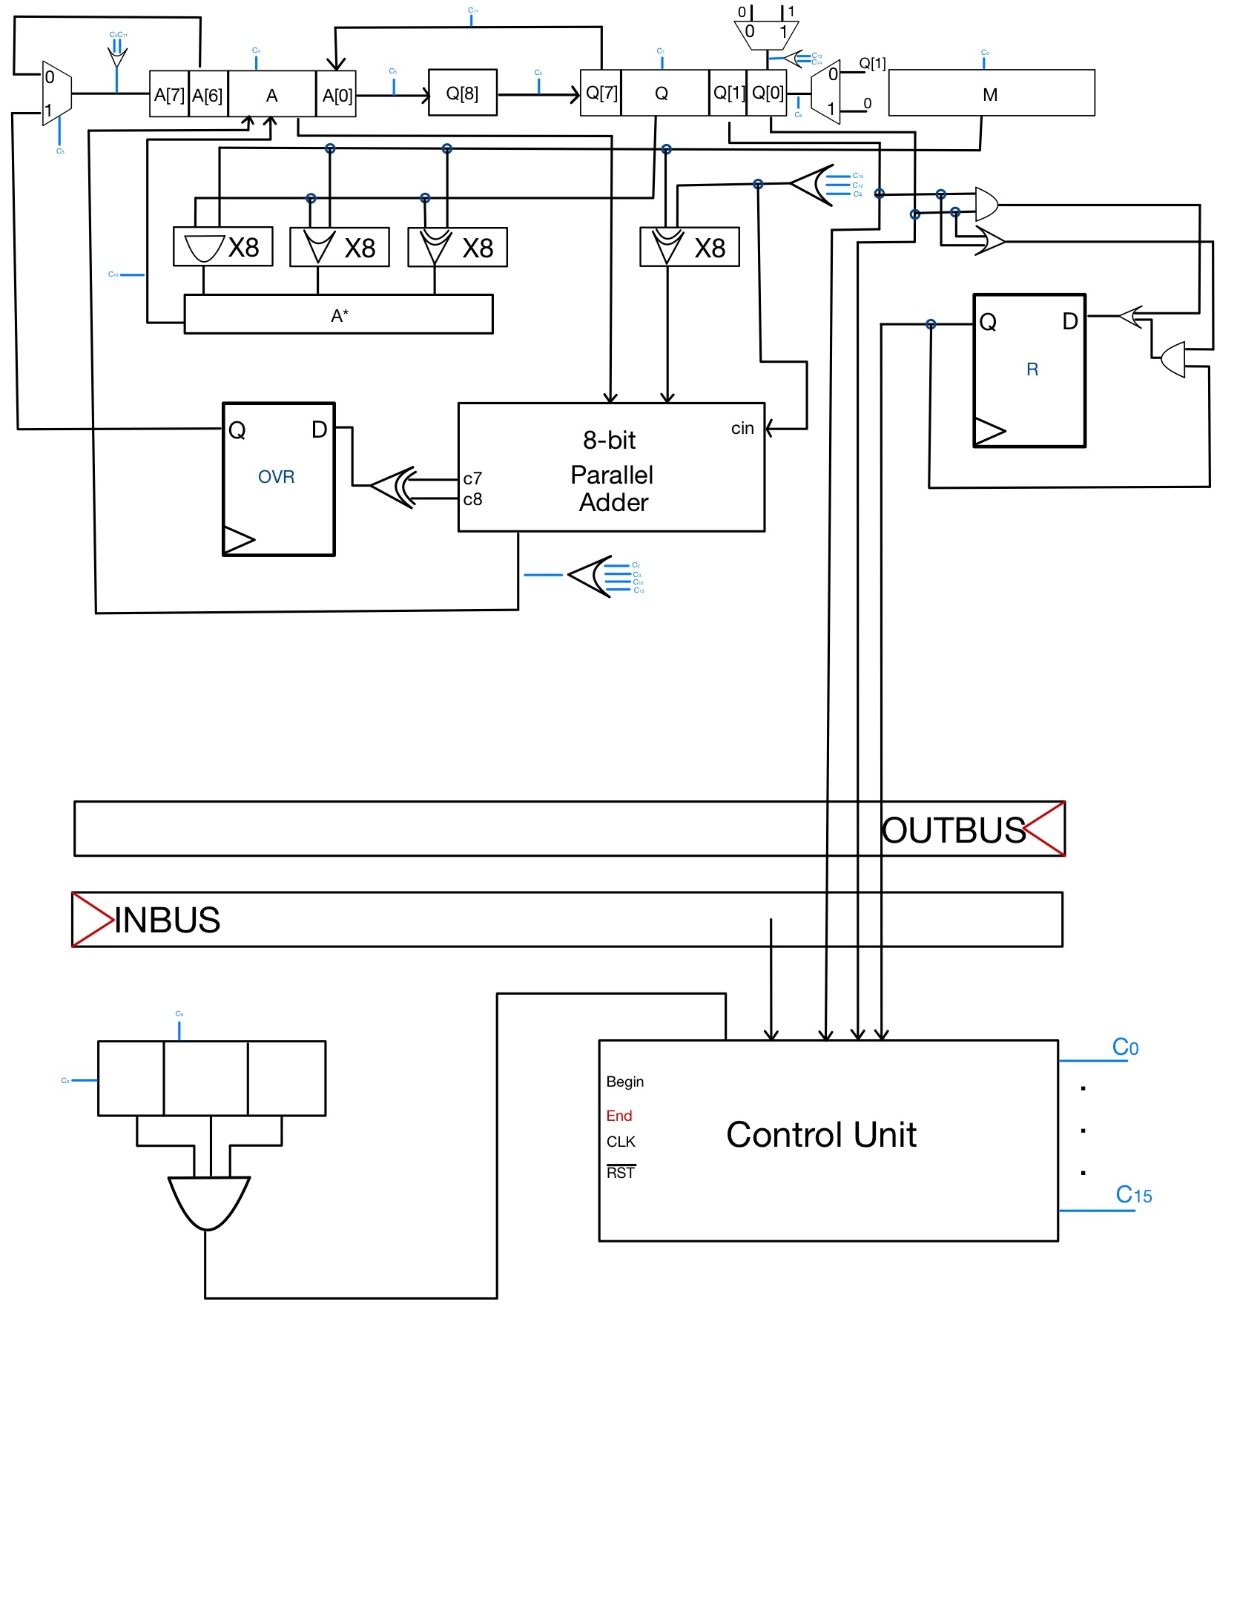
\includegraphics[scale=0.3]{Documentation/ALU}
\end{center}

When looked at from the inside, the ALU exposes a series of low-level hardware components that work together, under the guidance of the control signals
generated by the control unit, to implement each step of the chosen operation accordingly. The main elements at play here are the A, Q and M
\textbf{Universal Shift Registers}, used for storing both the values of the incoming operands and the partial results and also shift them if needed, the
\textbf{D-type Flip-Flops} used to store the two intermediate auxilliary states, the overflow flag (OVR), which tells us when the partial result of the
Modified Booth algorithm needs to undergo a correction step due to the limitations of modulo-n arithmetic, and the run-of-bits flag, R, also useful in
the context of Modified Booth, for taking advantage certain simplifications that help us skip through some of the arithmetic involved in doing multiplication,
the \textbf{8-bit Paralled Adder} that computes partial sums or differences, a suite of \textbf{logic gates} for the simple logical operations that are
multiplexed together and get computed all the time, \textbf{8-bit Input and Output Busses} used for delivering the data, both from the user to the hardware
and vice versa, and the \textbf{Control Unit} that takes into consideration the current state of the ALU machine (including a
\textbf{counter} for keeping the track of repetitive operations) in order to decide which signal to activate so that it helps with the transition into the next state.

\begin{center}
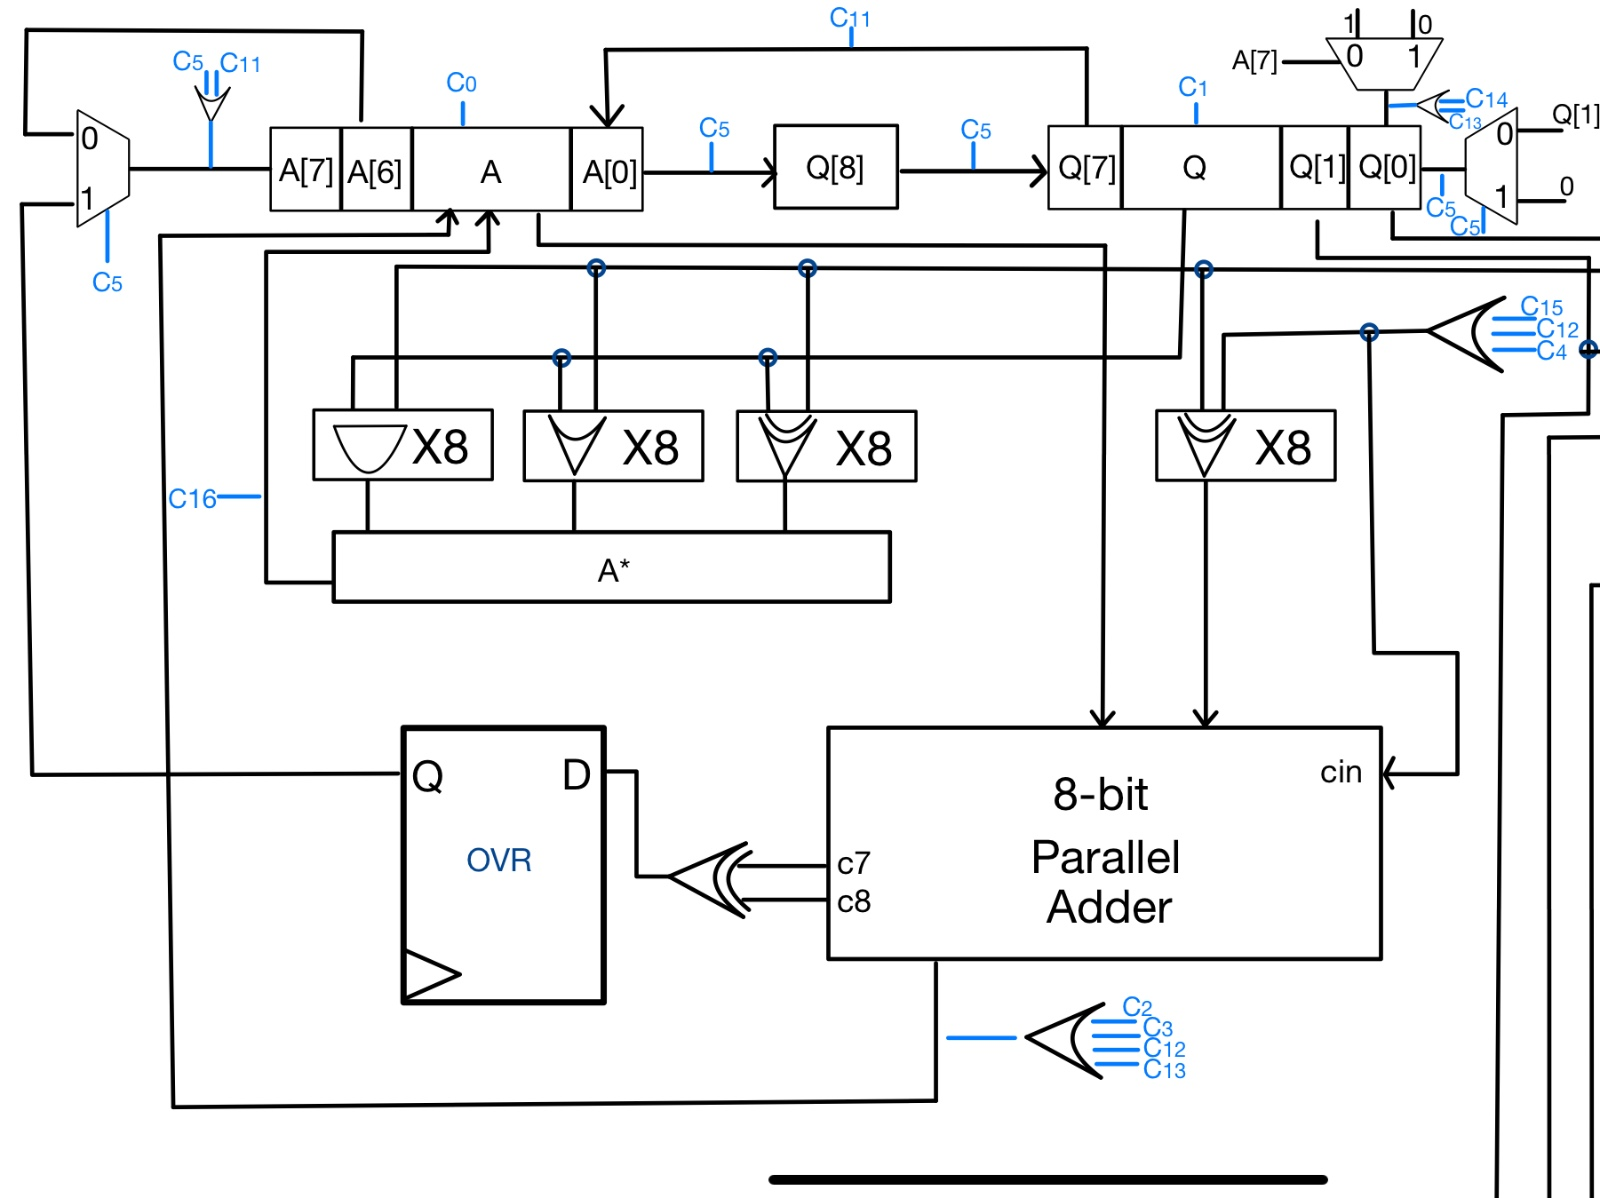
\includegraphics[scale=0.2]{Documentation/ALU1}
\end{center}

There are three registers used to handle loading, dispatching and alteration of data. The Q and M registers store the two operands required for each operation, and
in addition to them there's the A register that acts as an accumulator for partial results and also as an extension of the Q register, especially useful
for the expansion of the bit domain of the first operand, from 8-bit to 16-bit, when performing division. A and Q hold the final results, at the end of the
operation, and, depending on user selection, get concatenated to store the outcome of multiplication, are left separated for simple operations, case in which A stores the output
value, or represent the remainder and the quotient respectively, after the end of division. There's and additional D-type flip-flop, Q8, used to expand the bit
domain of Q when executing the Modified Booth algorithm.
The values stored are in two's complement, a storing
techinque for signed numbers that has the major advantage of preserving corectness of arithmetical operations, regardless of sign. These registers have both
the capacity to be loaded into in parallel fashion, meaning all 8 bits get stored simultaneously, within the same clock cycle, and to perform both left and right
shifting operations, required by the multiplication and division algorithms, meaning neighbouring bits get copied into one another, either from
left to right, or right to left, while the leftmost or rightmost bit gets overwritten by an external incoming bit, chosen in function of the current
operation and implicitly by the currently active control signal. This fundamental duality gives these hardware elements the name of universal shift registers. Their
logic design was mainly inspired by the implementation provided below. 

\begin{center}
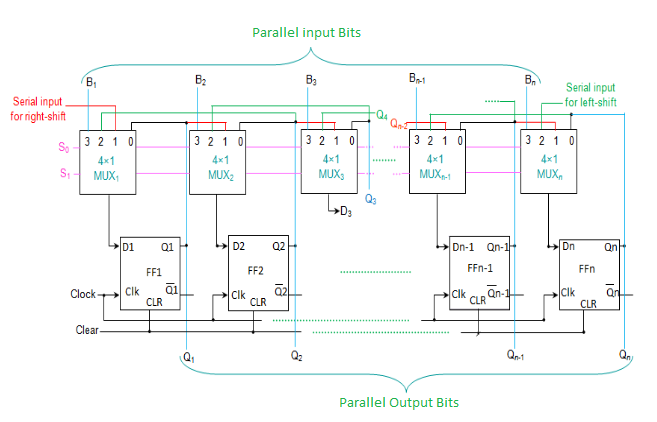
\includegraphics[scale=0.8]{Documentation/registers}
\end{center}

The modules situated right bellow the registers are simply an array of logic gates used to perform bit by bit logic operations between correspoding bits
of the operands. The result is then decidedly stored inside the $\text{A}^*$ temporary register, through an implicit multiplexer, waiting to be stored
inside A when the dedicated control signal is activated.\\

After that there is the Parallel Adder module. It is used for both subtraction and addition. It takes advantage of the following fact:

\[ a \text{ xor } 0 = a \]
\[ a \text{ xor } 1 = \overline{a} \]

and uses it to negate the second operand and add then 1 to it through the initial carry, which is essentialy two's complementing the operand, equivalent
to treating the expression $X - Y$ as $X + (-Y)$. It is then known that the state of the overflow flag can be computed as an exclusive or between
the last and next to last carries of the addition operation. The adder chosen for this ALU is a Ripple Carry Adder (RCA):

\begin{center}
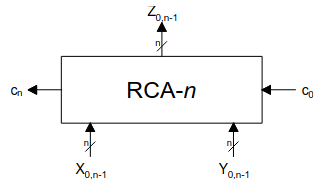
\includegraphics[scale=0.5]{Documentation/RCA}
\end{center}

An n-bit RCA is an abstraction of n concatenated Full Adder Cells (FACs), each capable of performing 1-bit addition, including computing the carry.

\begin{center}
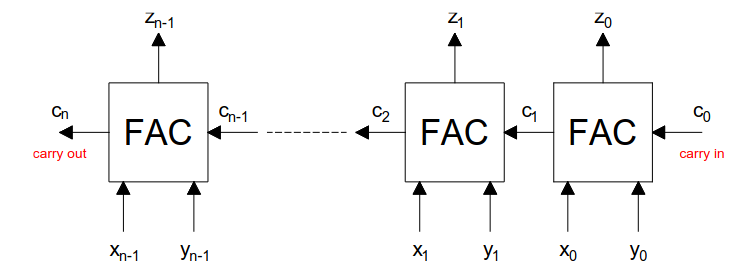
\includegraphics[scale=0.5]{Documentation/FACs}
\end{center}

The standard hardware implementation of a FAC is provided below.

\begin{center}
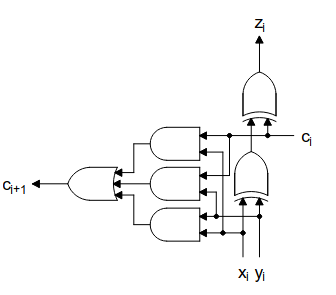
\includegraphics[scale=0.5]{Documentation/FAC}
\end{center}

\begin{center}
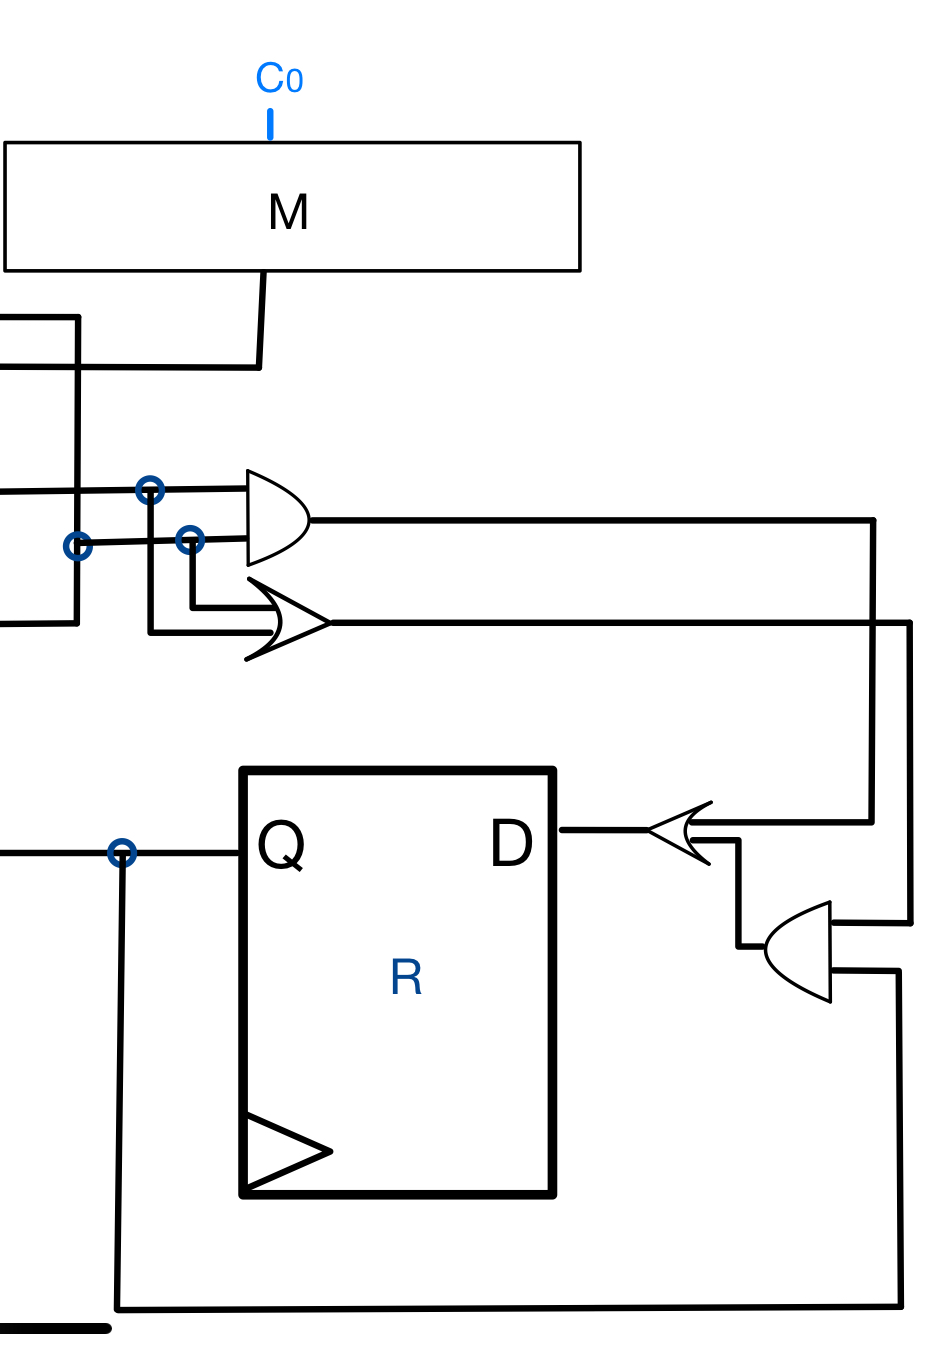
\includegraphics[scale=0.3]{Documentation/ALU2}
\end{center}

The R flag is determined by the formula

\[ R_n = x_1x_0 + R_{n - 1}(x_1 + x_0), \]

which tells us whether we are in the middle, at the beginning, or at the end of a run of 1 bits, case in which we are going to perform the operation
decided by the control unit, in accordance with the steps of the Modifiend Booth algorithm.

\begin{center}
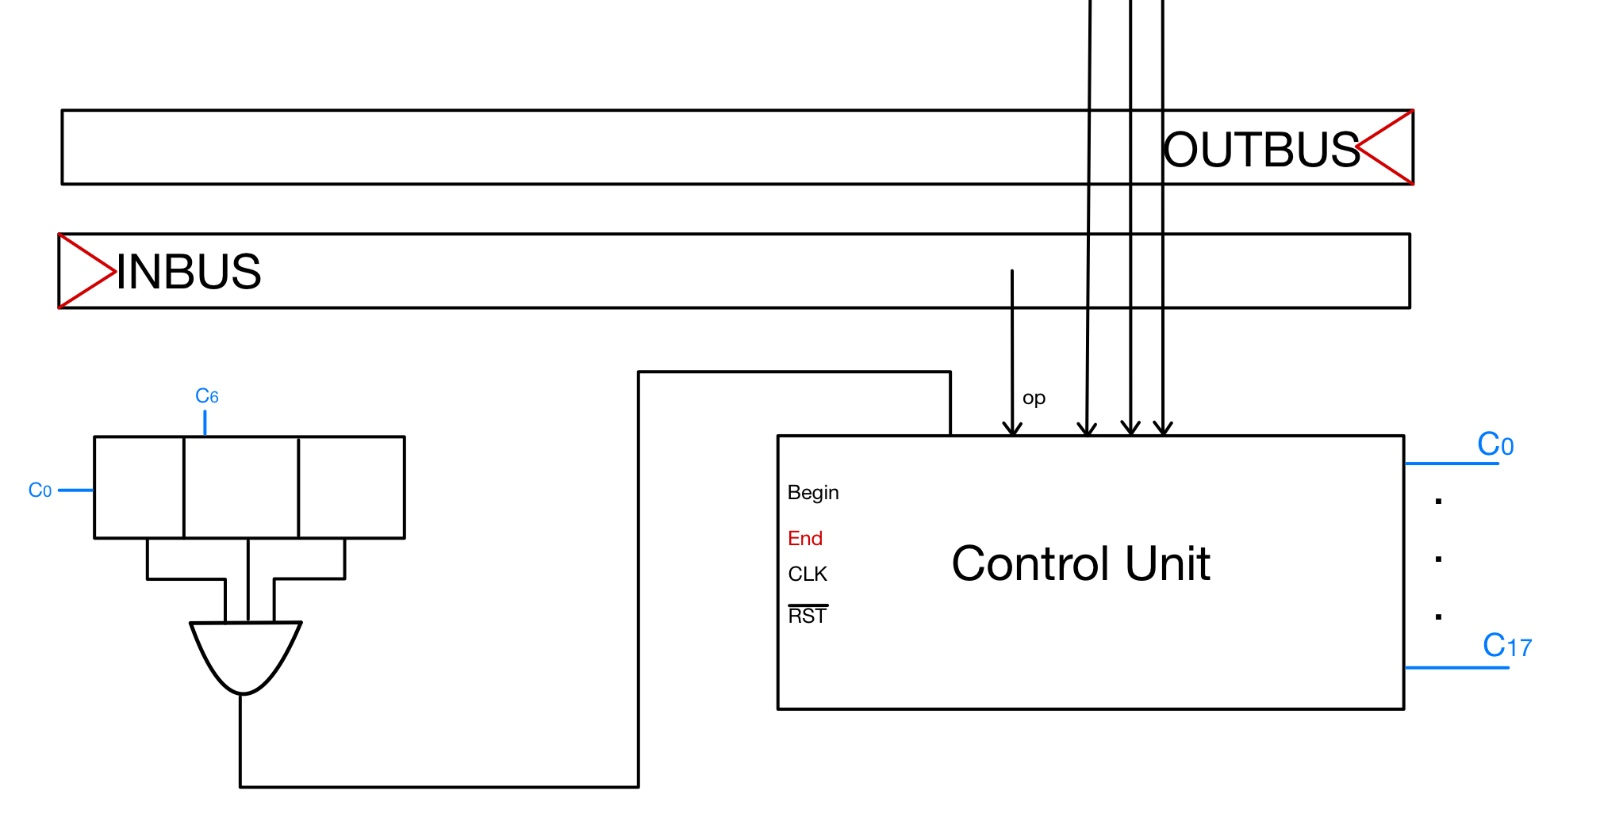
\includegraphics[scale=0.3]{Documentation/ALU3}
\end{center}

The counter is there to make sure we perform exactly 8 steps of the looping parts in the Modified Booth and Restoring Division algorithms, one for each bit
of the operand. It simply counts from 0 to 7 and then it resets its value back to 0. The incrementation happens when its internal \textit{count up} signal
is activated (concretely, the \textit{count up} signal is sent by the control unit, at the end of each repetitive step). It is implemented using
T-type flip-flops, that toggle recursively, whenever the previous digits of the counter reach together the maximum value up to that order of
magnitude.\\

\begin{center}
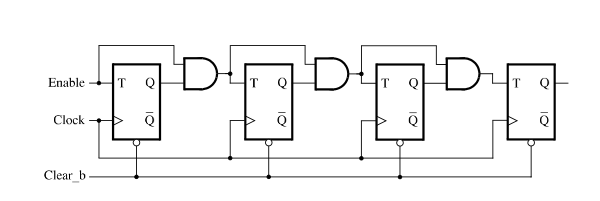
\includegraphics[scale=0.6]{Documentation/counter}
\end{center}

The control unit is the single most complex and non-standard, in regards to implementation, component of the ALU system, and therefore is going to be
discussed in great detail in its own separate section.

\Section{5}{Control Unit}

The control unit is a key component of the ALU system, responsible for coordinating the execution of operations by generating the necessary control signals at each step. In this project, the control logic is implemented using a
sequence counter, which acts as a simple state machine. Each state corresponds to a specific stage in the execution process, such as loading operands, performing the selected operation, or storing the result. By advancing through
its states in a predefined order, the sequence counter ensures that all operations are carried out in the correct sequence and with proper timing. This approach simplifies the control logic and makes the overall system easier to
manage and debug.\\

To implement the control logic, a \textcolor{YellowGreen}{Modulo-5-sequence} counter was designed, which cycles through five distinct states corresponding to the stages of the ALU operation.
This module serves as the core timing mechanism of the control
unit. The system is composed of several interconnected submodules:
\textcolor{YellowGreen}{Decoder-1-out-of-5}, a \textcolor{YellowGreen}{Modulo-5-counter}, and an \textcolor{YellowGreen}{SR flip-flop}. Each component plays a specific role in generating and controlling the state transitions.\\

1. \textcolor{YellowGreen}{\textbf{Modulo-5-counter}}

This module generates a repetitive sequence of five binary values (from 0 to 4) that represent the current phase. It increments its output on each clock cycle, looping back to zero after reaching four. The modulo-5 behavior
ensures that the control unit progresses through exactly five phases before restarting the sequence.\\

2. \textcolor{YellowGreen}{\textbf{Decoder-1-out-of-5}}

The decoder takes the 3-bit output from the modulo-five counter and activates exactly one of its five outputs at a time. This ensures that only one phase signal is active during each step, allowing precise control over which
control lines are enabled. Essentially, it translates the binary count into a one-hot encoding format, which is easier to use for controlling sequential logic.\\

3. \textcolor{YellowGreen}{\textbf{SR Flip-Flop}}

The Start/Stop latch controls whether the sequence counter is active or halted. It enables or disables the advancement through the counting sequence based on external conditions or control inputs. When the latch is set, the
modulo-5 counter is allowed to advance on each clock cycle, progressing through the defined control states. When reset, the counter is held in place, effectively pausing the control unit. This mechanism provides a simple and
effective way to synchronize the ALU's operation with the system's global control logic.

\begin{center}
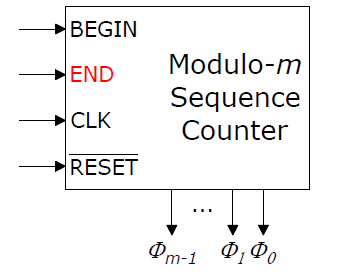
\includegraphics[scale=0.3]{Documentation/modulo_counter}
\end{center}

The picture illustrates the internal structure and signal connections within the \textcolor{YellowGreen}{Modulo-5-sequence} counter used in the control unit.
It shows how the \textcolor{YellowGreen}{Modulo-5-counter}, \textcolor{YellowGreen}{1-out-of-5 Decoder} and the \textcolor{YellowGreen}{Start/Stop} latch are connected to
manage state transitions. 


\begin{center}
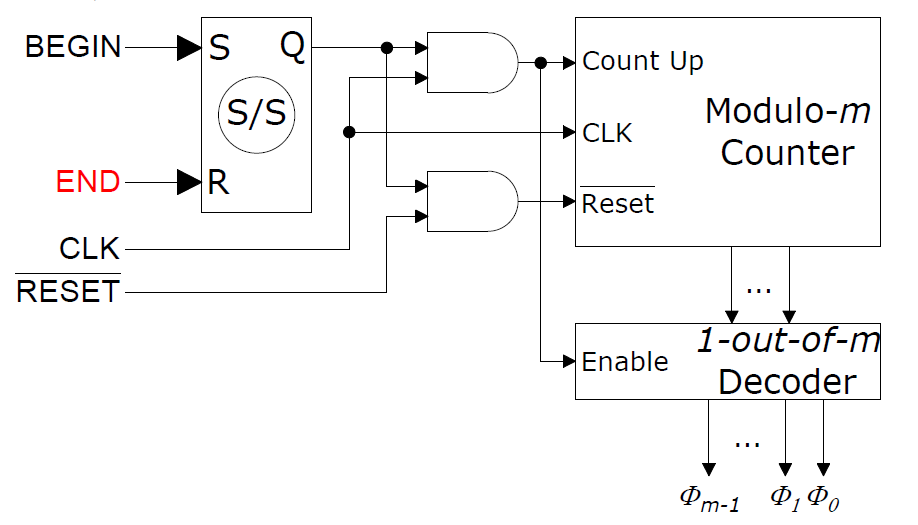
\includegraphics[scale=0.3]{Documentation/sr}
\end{center}

Each operation supported by the ALU has a specific set of control signals that are activated during certain steps of the control sequence. These signals coordinate actions such as loading operands, enabling the ALU,
performing addition or subtraction, and storing the result. The list below outlines the control signals associated with each operation and indicates during which phase (based on the output of the Modulo-5 sequence counter) each
signal is active:\\

\textcolor{ForestGreen}{\textbf{Control Signals by Operation}}\\

1. \textcolor{red}{AND} / \textcolor{red}{OR} / \textcolor{red}{XOR} (Logical Operations)\\

Operation codes: \textcolor{red}{AND}(\textcolor{ForestGreen}{000}), \textcolor{red}{AND}(\textcolor{ForestGreen}{001}), \textcolor{red}{XOR}(\textcolor{ForestGreen}{010})\\

Cycle 0: 

\begin{itemize}
  \item Phase 0: \textcolor{cyan}{c0} -> Load operand M
  \item Phase 1: \textcolor{cyan}{c1} -> Load operand Q
  \item Phase 2: \textcolor{cyan}{c2} -> Enable logic unit
  \item Phase 3: \textcolor{cyan}{c16} -> Store result in A-star based of off op
\end{itemize}


Cycle 9:

\begin{itemize}
  \item Phase 0: \textcolor{cyan}{c7} -> Load result A
  \item Phase 1: \textcolor{cyan}{c8} -> Load result Q
\end{itemize}
---------> Activate \textcolor{red}{END} signal\\

2. \textcolor{BurntOrange}{ADD} / \textcolor{BurntOrange}{SUB} (Arithmetic Operations)\\

Operation codes: \textcolor{BurntOrange}{ADD}(\textcolor{ForestGreen}{011}), \textcolor{BurntOrange}{SUB}(\textcolor{ForestGreen}{100})\\

Cycle 0:

\begin{itemize}
  \item Phase 0: \textcolor{cyan}{c0} -> Load operand M
  \item Phase 1: \textcolor{cyan}{c1} -> Load operand Q
  \item Phase 2: \textcolor{cyan}{c2} -> Triggers addition, the result is stored in A
  \item Phase 2: \textcolor{cyan}{c15} -> Triggers subtraction, the result is stored in A
\end{itemize}


Cycle 9:

\begin{itemize}
  \item Phase 0: \textcolor{cyan}{c7} -> Load result A
  \item Phase 1: \textcolor{cyan}{c8} -> Load result Q
\end{itemize}
---------> Activate \textcolor{red}{END} signal\\

3. \textcolor{purple}{MULTIPLICATION} (Modified Booth)\\

Operation codes: \textcolor{purple}{MULTIPLICATION}(\textcolor{ForestGreen}{101})\\

Cycle 0:

\begin{itemize} \item Phase 0: \textcolor{cyan}{c0} -> Load operand M and initialize A, COUNT, R, OVR \item Phase 1: \textcolor{cyan}{c1} -> Load operand Q and Q8 \end{itemize}

Cycle 1 - 8:

\begin{itemize} \item Phase 0: \textcolor{cyan}{c3} -> Triggers addition for Q1Q0R in {001, 010, 101, 110}, R* = 0, OVR is calculated \item Phase 0: \textcolor{cyan}{c4} -> Additional signal for subtraction for Q1Q0R in {101, 110}, R* = 1, OVR is calculated \item Phase 1: \textcolor{cyan}{c5} -> Triggers right shift \item Phase 2: \textcolor{cyan}{c6} -> COUNT is updated \end{itemize}

Cycle 9:

\begin{itemize} \item Phase 0: \textcolor{cyan}{c7} -> Load result A \item Phase 0: \textcolor{cyan}{c5} -> Triggers final right shift \item Phase 1: \textcolor{cyan}{c8} -> Load result Q \end{itemize} ---------> Activate \textcolor{red}{END} signal\\

4. \textcolor{purple}{DIVISION} (Restoring Division)\\

Operation codes: \textcolor{purple}{DIVISION}(\textcolor{ForestGreen}{110})\\

Cycle 0:

\begin{itemize} \item Phase 0: \textcolor{cyan}{c0} -> Load operand M \item Phase 1: \textcolor{cyan}{c1} -> Load operand Q \item Phase 2: \textcolor{cyan}{c10} -> Load operand A (first half of the dividend) \item Phase 3: \textcolor{cyan}{c11} -> Triggers initial left shift \end{itemize}

Cycle 1 - 8:

\begin{itemize} \item Phase 0: \textcolor{cyan}{c12} -> Triggers subtraction \item Phase 1: \textcolor{cyan}{c13} -> Triggers addition when A[7] = 1, updates Q[0] = 0 \item Phase 1: \textcolor{cyan}{c14} -> Updates Q[0] = 1 \item Phase 2: \textcolor{cyan}{c6} -> COUNT is updated \item Phase 3: \textcolor{cyan}{c17} -> Triggers left shift \end{itemize}

Cycle 9:

\begin{itemize} \item Phase 0: \textcolor{cyan}{c7} -> Load result A \item Phase 0: \textcolor{cyan}{c9} -> Load result Q \end{itemize} ---------> Activate \textcolor{red}{END} signal\\

\textbf{Observation}: Phase 4 is consistently used as the transition point between cycles.\\

The control unit is built using a \textcolor{YellowGreen}{Modulo-5-Sequence-Counter} and a set of three SR flip-flops, which together manage the execution flow of each operation. The sequence counter generates the control phases, cycling through 5 phases. At the same time, the SR flip-flops hold the information about which cycle is currently being executed.
Depending on the combination of the
current phase (given by the counter) and the active cycle (stored in the SR-FFs), the system activates specific control signals. This structure ensures that, for each operation type, only the required control lines are triggered at the correct moment during execution.\\


\begin{center}
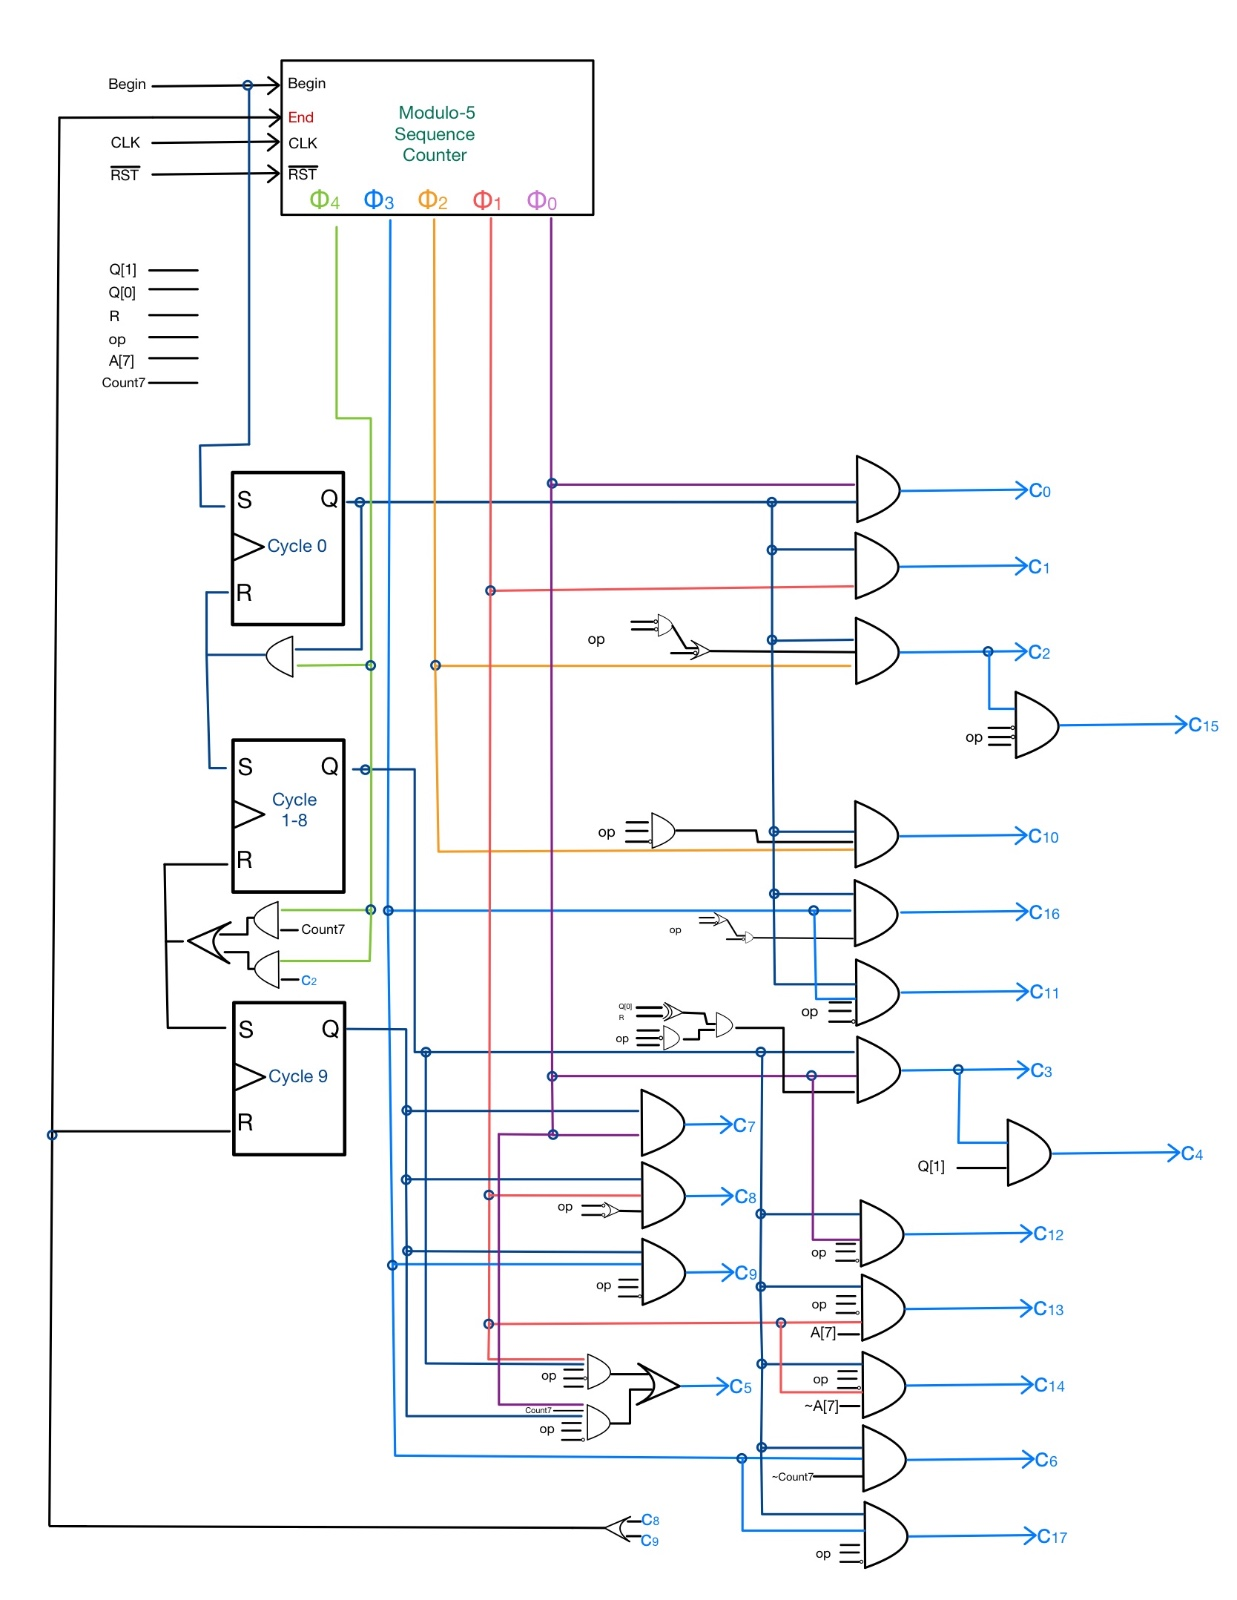
\includegraphics[scale=0.3]{Documentation/control_unit}
\end{center}

\Section{6}{Results}

To illustrate the functionality of the ALU, each supported operation is presented below along with its corresponding operation code (opcode) and a simulation result. These examples provide a visual and practical understanding of how the ALU processes 8-bit operands to perform logical and arithmetic computations.\\

1. \textbf{AND Operation}
\textbf{Opcode}: \textcolor{ForestGreen}{000}
The AND operation performs a bitwise conjunction between the two 8-bit operands. Each bit in the result is set to 1 only if the corresponding bits in both inputs are 1. The simulation output confirms this behavior, showing the correct result where only common bits are preserved.
For example, if \textbf{X = 17 (0001 0001)} and \textbf{Y = 5 (0000 0101)}, the result of the operation is                   \textbf{$OUT_A$ = 1 (0000 0001)}, which is highlighted in green in the simulation image.

\begin{center}
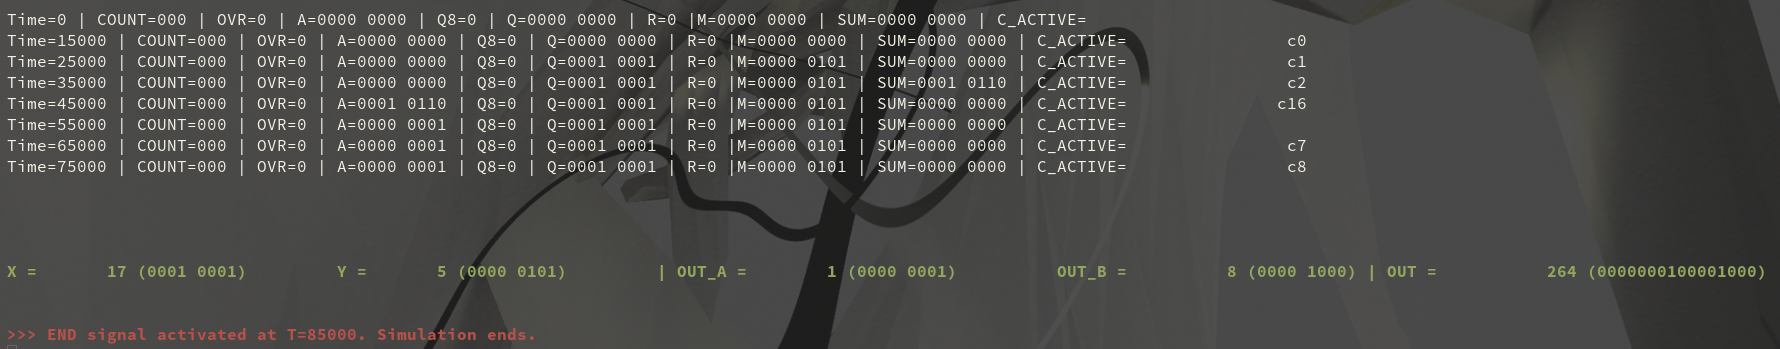
\includegraphics[scale=0.3]{Documentation/AND}
\end{center}

2. \textbf{OR Operation}
\textbf{Opcode}: \textcolor{ForestGreen}{001}
The OR operation performs a bitwise disjunction between the operands. In the output, a bit is 1 if it is set in either of the input operands. The simulation result highlights how the operation combines the inputs, setting bits wherever at least one input has a 1.
For example, if \textbf{X = 17 (0001 0001)} and \textbf{Y = 5 (0000 0101)}, the result of the operation is \textbf{$OUT_A$ = 21 (0001 0101)}, which is highlighted in green in the simulation image.

\begin{center}
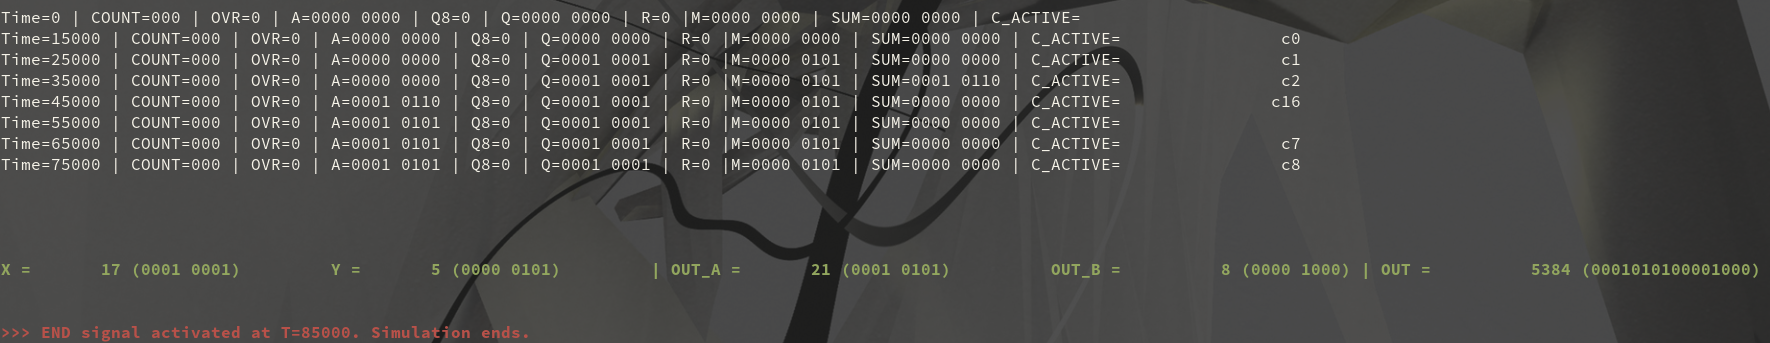
\includegraphics[scale=0.3]{Documentation/OR}
\end{center}

3.     \textbf{XOR Operation}
    \textbf{Opcode}: \textcolor{ForestGreen}{010}
    This operation executes a bitwise exclusive OR. A bit in the result is 1 if the corresponding bits in the operands are different. The output correctly reflects this rule, demonstrating how the XOR operation highlights differences between the inputs.
    For example, if \textbf{X = 17 (0001 0001)} and \textbf{Y = 5 (0000 0101)}, the result of the operation is \textbf{$OUT_A$ = 20 (0001 0100)}, which is highlighted in green in the simulation image.

\begin{center}
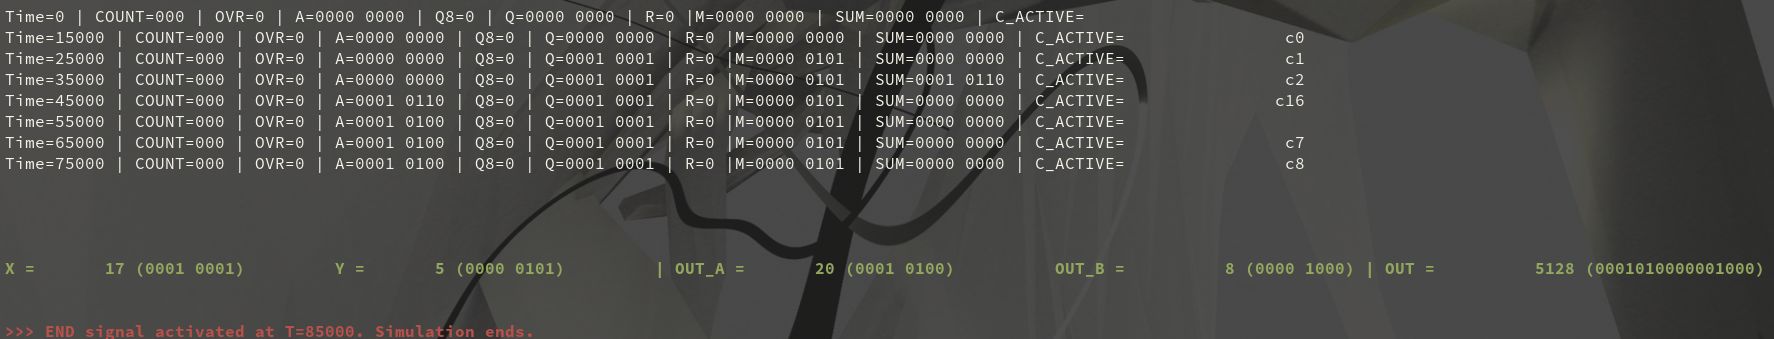
\includegraphics[scale=0.3]{Documentation/XOR}
\end{center}

4. \textbf{ADD Operation}
\textbf{Opcode}: \textcolor{ForestGreen}{011}
The ADD operation computes the sum of the two 8-bit operands, with carry propagation across bits. The addition is performed using a Ripple Carry Adder (RCA), a simple yet effective design where each bit's carry is passed to the next stage sequentially.
For example, if \textbf{X = 17 (0001 0001)} and \textbf{Y = 5 (0000 0101)}, the result of the operation is \textbf{$OUT_A$ = 22 (0001 0110)}, which is highlighted in green in the simulation image.

\begin{center}
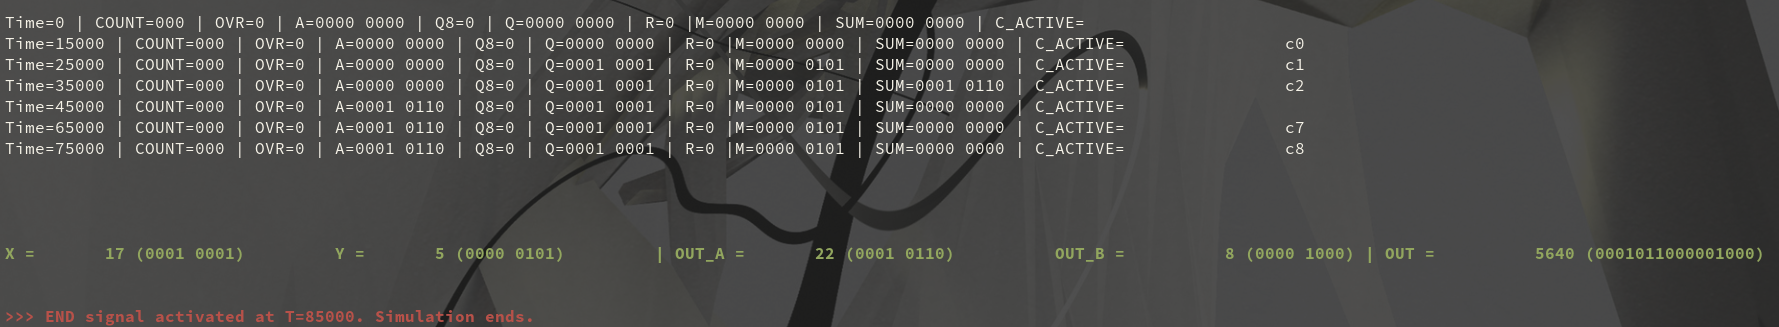
\includegraphics[scale=0.3]{Documentation/ADD}
\end{center}

5.     \textbf{SUB Operation}
    \textbf{Opcode}: \textcolor{ForestGreen}{100}
    The SUB operation subtracts the second operand from the first using two’s complement arithmetic. This operation also uses a Ripple Carry Adder (RCA), similar to the ADD operation. However, before entering the adder, the second operand is passed through an XOR gate to invert its bits, and the carry-in (Cin) of the adder is set to 1.
    For example, if \textbf{X = 17 (0001 0001)} and \textbf{Y = 5 (0000 0101)}, the result of the operation is \textbf{$OUT_A$ = 12 (0000 1100)}, which is highlighted in green in the simulation image.

\begin{center}
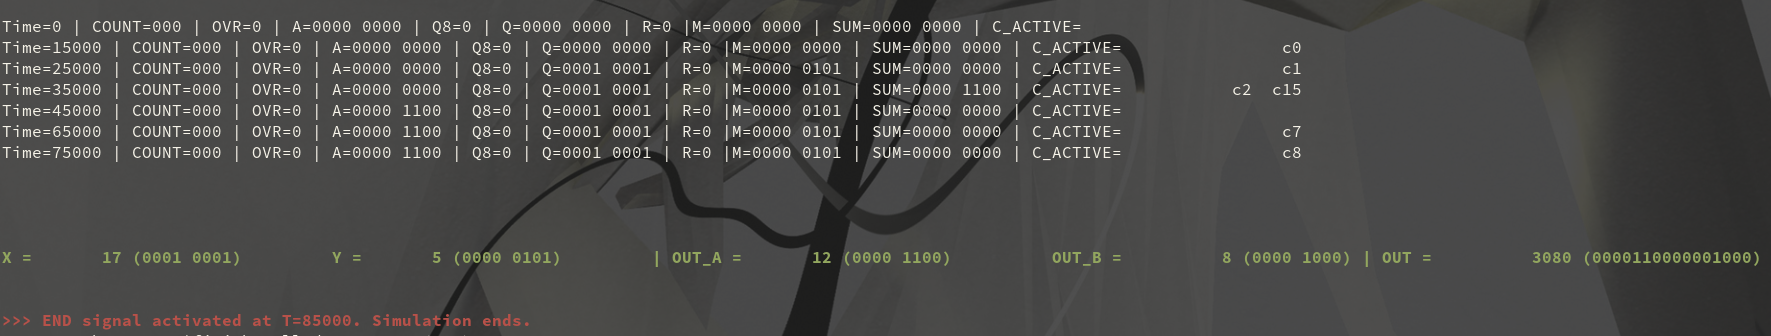
\includegraphics[scale=0.3]{Documentation/SUB}
\end{center}


6.     \textbf{MUL Operation (Modified Booth)}
    \textbf{Opcode}: \textcolor{ForestGreen}{101}
    This operation performs multiplication using the Modified Booth algorithm, efficiently handling signed numbers. The output from the simulation confirms the algorithm's correct implementation, showing a 16-bit result as the product of two 8-bit signed numbers.
    For example, if \textbf{X = -71 (1011 1001)} and \textbf{Y = -123 (1000 0101)}, the result of the operation is \textbf{OUT = 8733 (0010 0010 0001 1101)}, which is highlighted in green in the simulation image.

\begin{center}
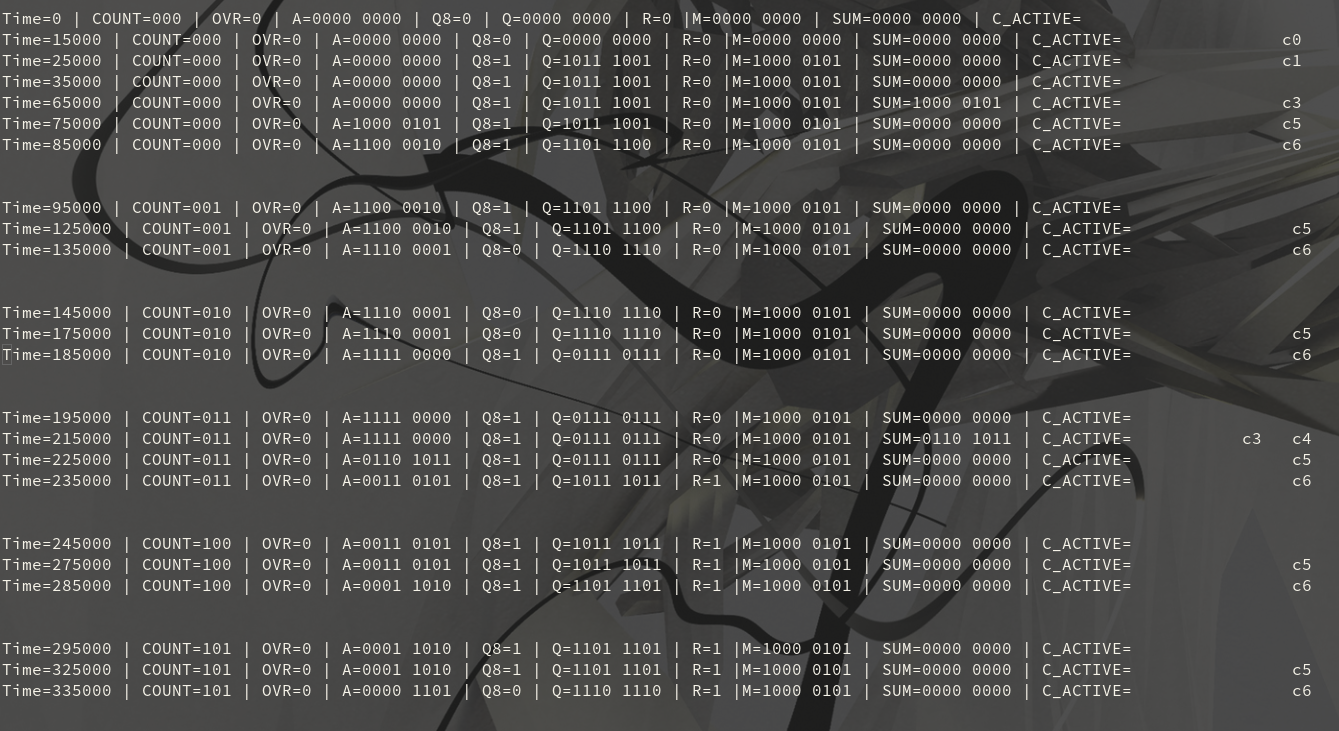
\includegraphics[scale=0.3]{Documentation/MUL1}
\end{center}

\begin{center}
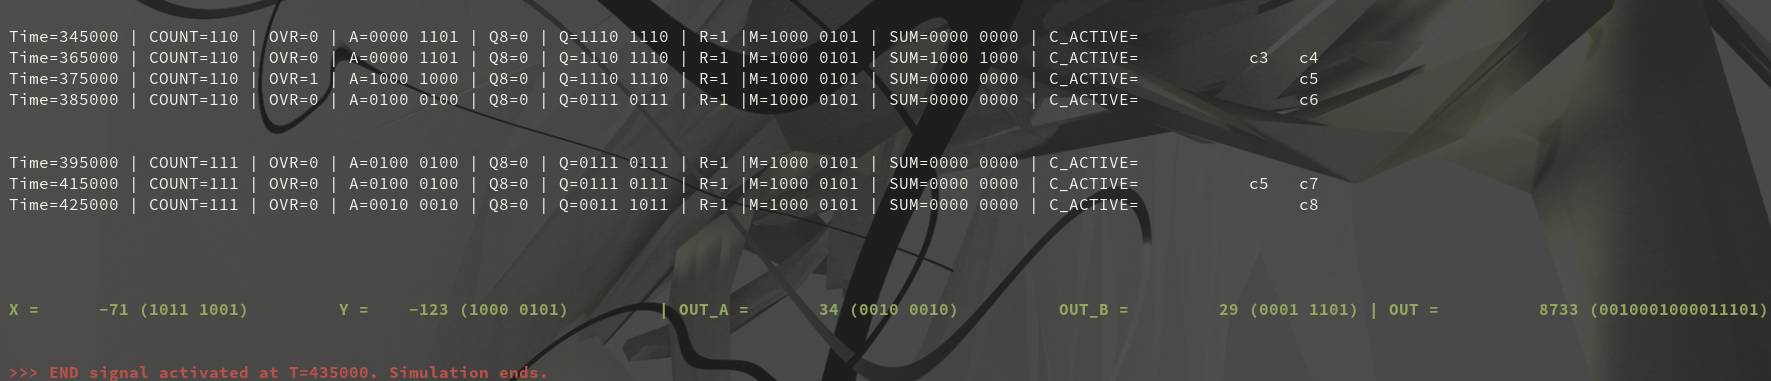
\includegraphics[scale=0.3]{Documentation/MUL2}
\end{center}

7. \textbf{DIV Operation (Restoring Division)}
\textbf{Opcode}: \textcolor{ForestGreen}{110}
The DIV operation carries out division using the restoring division method. The simulation displays the correct quotient and remainder, split across separate registers or outputs.
For example, if \textbf{X = 5771 (0001 0110 1000 1011)} and \textbf{Y = 135 (1000 0111)}, the result of the operation is \textbf{REMAINDER = 101 (0110 0101)} and \textbf{QUOTIENT = 42 (0010 1010)}, which is highlighted in green in the simulation image.

\begin{center}
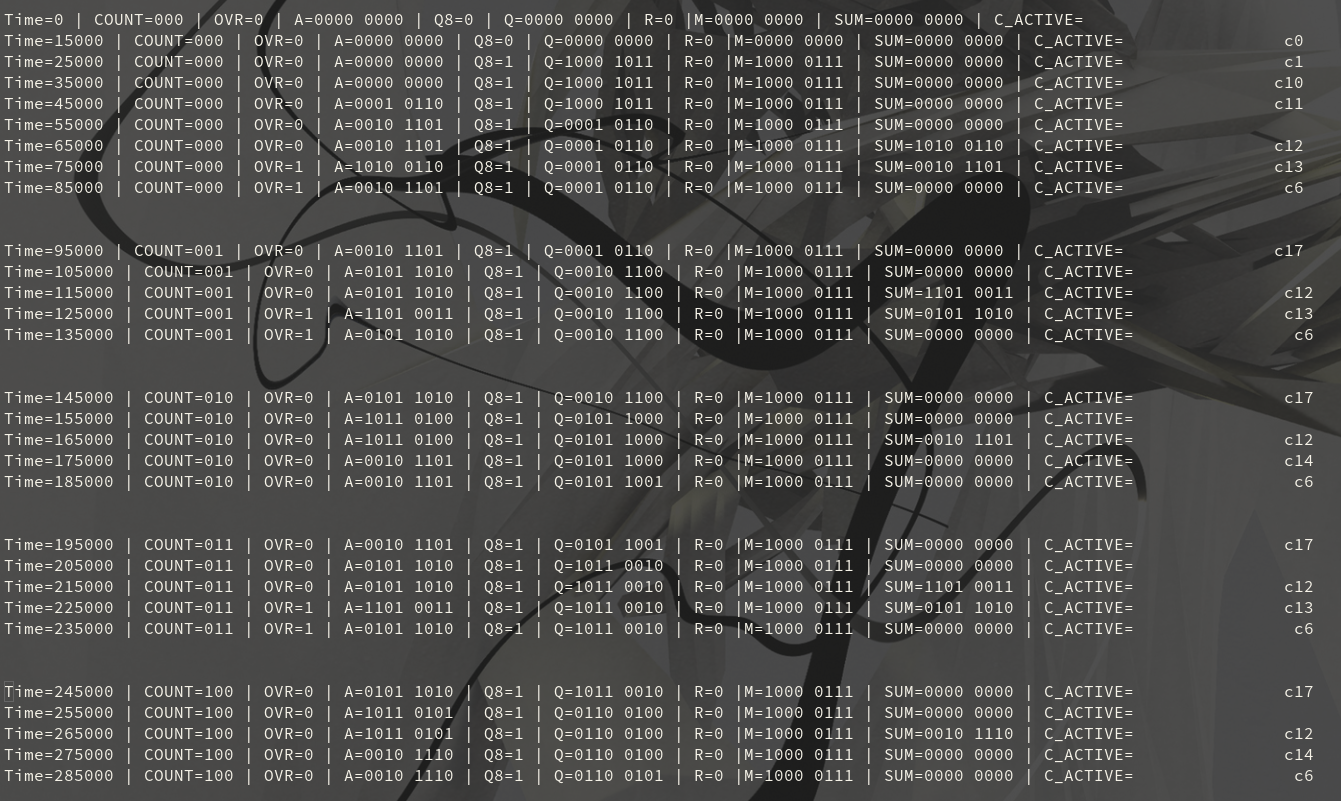
\includegraphics[scale=0.3]{Documentation/DIV1}
\end{center}

\begin{center}
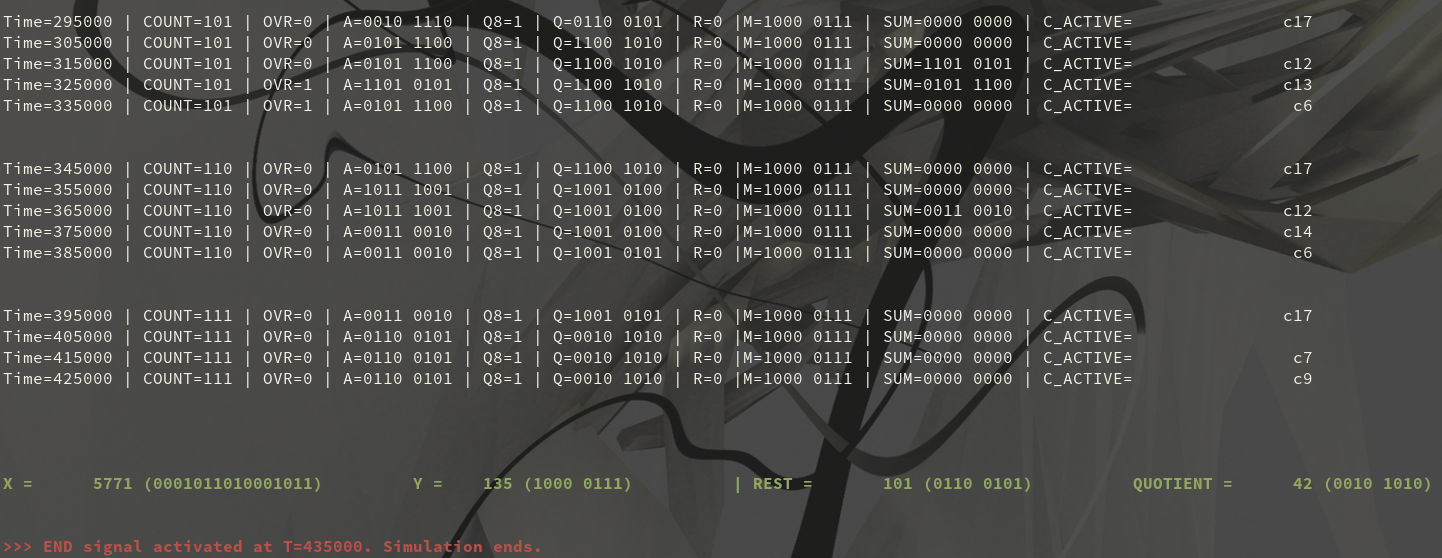
\includegraphics[scale=0.3]{Documentation/DIV2}
\end{center}

\newpage

\Section{7}{Bibliography}

\textbf{Tools Used}:\\

\textbf{EDAPlayground} – utilized for writing, testing, and simulating the code in a web-based environment.\\

\textbf{Icarus Verilog (iverilog)} – used as the underlying simulation engine for compiling and running Verilog code on a local machine.\\

\textbf{Canva} – used to create clear and visually structured diagrams that support the explanation of the design flow.\\

\textbf{ChatGPT} – assisted in drafting and refining the written content to ensure clarity and coherence.\\

\textbf{Bibliography}:\\

Oprițoiu Flavius, (2025) Computer Architecture, Polytechnic University of Timișoara\\
https://www.geeksforgeeks.org/universal-shift-register-in-digital-logic/

\end{document}
